\subsection{終対象}
  対象の元で述べた終対象は実は普遍性で定義される。積の普遍性と似ているようで似ていない雰囲気であるが、
	\begin{define}[終対象]
		ある圏$\cat{C}$に\textbf{終対象}が存在するとは、ある対象$1$が存在して圏$\cat{C}$の任意の対象$X$に対し射$\mor{!_X}{X}{1}$が\textbf{一意}に\textbf{存在}するときである。

		元を取る操作とは射の向きが逆であることに注意してほしい。
	\end{define}
  積対象$A\times B$はある対象$A,B$や二つの射影射に対して定義されるのであったが、終対象は既存の対象や射に対して定義されるものではない。後に証明するが、一つの圏に対して一つの終対象を考えると捉えて良い。\\
	また同様に射の対$\mor{\tuple{f,g}}{X}{A\times B}$は対象$X$と射$f,g$に対して一意に存在するのであったが、終対象への射$\mor{!_X}{X}{1}$は対応する射が存在しない。そのため、終対象への射は対象$X$に対して無条件で一意に存在することになる。
	\begin{prop}[終対象から終対象への射]
		終対象から終対象への射は恒等射ただ一つである。
	\end{prop}
	\begin{proof}
		終対象$1$に対して、終対象から終対象への射$\mor{!_1}{1}{1}$は無条件で一意に定まる。
		すべての対象に恒等射は存在するから$id_1=!_1$となる。
		\begin{center}
			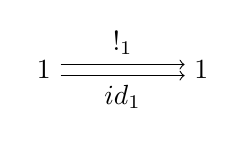
\begin{tikzpicture}[auto]
				\node (1) at (0, 0) {$1$};
				\node (1') at (2, 0) {$1$};
				\draw[->,transform canvas={yshift=2pt}] (1) to node{$!_{1}$}(1');
				\draw[->,transform canvas={yshift=-2pt}] (1) to node[swap]{$id_1$}(1');
			\end{tikzpicture}
		\end{center}
	\end{proof}

	\begin{prop}[終対象の一意性]
		終対象$1$に対して別の終対象$I$が存在するとき、$1\cong I$が成り立つ。すなわち終対象は\textbf{同型を除いて一意}に定まる。
	\end{prop}
	\begin{proof}
		終対象$1$における$I$からの一意に定まる射$\mor{!_I}{I}{1}$と終対象$I$における$1$からの一意に定まる射$\mor{i_1}{1}{I}$の合成$\mor{!_I\circ i_1}{1}{1}$と$\mor{i_1\circ!_I}{I}{I}$はそれぞれ終対象から終対象への射である。

		よって$!_I\circ i_1=id_1$と$i_1\circ!_I=id_I$が成り立ち、$!_I$、$i_1$が同型射になるから$1\cong I$が成り立つ。
		\begin{center}
			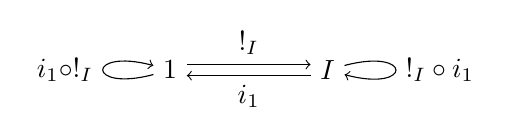
\begin{tikzpicture}[auto]
				\node (1) at (0, 0) {$1$};
				\node (1') at (2, 0) {$I$};
				\draw[->,transform canvas={yshift=2pt}] (1) to node{$!_I$}(1');
				\draw[->,transform canvas={yshift=-2pt}] (1') to node{$i_1$}(1);
				\draw[->,loop left ,looseness=20] (1) to node{$i_1\circ !_I$}(1);
				\draw[->,loop right ,looseness=20] (1') to node{$!_I\circ i_1$}(1');
			\end{tikzpicture}
		\end{center}
	\end{proof}

  最後に終対象と積の二つの普遍性を使った証明を考える。もし余力があれば自力で証明を書いてみてほしい。
  \begin{prop}[終対象との積]
    終対象$1$と任意の対象$A$において、$A\times 1\cong A$が成り立つ。
  \end{prop}
  \begin{proof}
    対象$A$が$1$と$A$に対する積対象であることを示せば良い。より正確には積$(A,id_A,!_A)$が$1,A$に対する積であることを示す。
    また、積$(A,id_A,!_A)$の任意の対象$X$からの二射$\mor{f}{X}{A}$、$\mor{!_X}{X}{1}$に対する射の対を$\mor{f}{X}{A}$とする。
    
    \begin{center}
			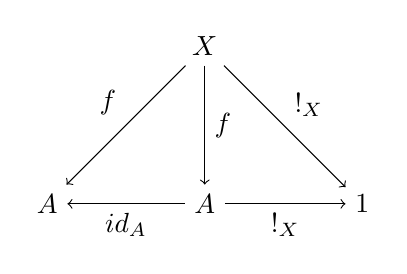
\begin{tikzpicture}[auto]
				\node (a) at (0, 0) {$A$};
				\node (ab) at (2, 0) {$A$};
				\node (b) at (4, 0) {$1$};
				\node (p) at (2, 2) {$X$};
				\draw[->] (p) to node[swap]{$f$}(a);
				\draw[->] (p) to node{$!_X$}(b);
				\draw[->] (p) to node{$f$}(ab);
				\draw[->] (ab) to node{$id_A$}(a);
				\draw[->] (ab) to node[swap]{$!_X$}(b);
			\end{tikzpicture}
    \end{center}

    まずは$f$が射の対であることを確認する。
    \begin{align*}
      id_A\circ f &= f&\text{(恒等射の定義)}\\
      !_A\circ f &= !_X&\text{(終対象の普遍性)}
    \end{align*}
    後者の式は$\mor{!_A\circ f}{X}{1}$と$\mor{!_X}{X}{1}$のどちらも対象$X$からの射であるため、終対象の定義より一意に定まる。よって$f$は確かに$f$と$!_X$の射の対である。

    次に射の対の一意性を示す。
    まずは$f$が射の対であることを確認する。
    同様に$f$と$!_X$の射の対となるような任意の射$f'$は以下の等式を満たす。
    \begin{align*}
      id_A\circ f' &= f\\
      !_A\circ f' &= !_X
    \end{align*}
    前者の等式より、$id_A\circ f'=f'=f$となり、射の対は一意に定まる。

    よって積$(A,id_A,!_A)$は$1$と$A$に対する積であり、積の一意性より$A\times 1\cong A$が成り立つ。

    また証明は省略するが、同型射はそれぞれ$\mor{\tuple{id_A,!_X}}{A}{A\times 1}$、$\mor{\pi_A}{A\times 1}{A}$となる。
  \end{proof}